\documentclass[handout,nooutcomes]{ximera}
%% handout
%% space
%% newpage
%% numbers
%% nooutcomes

%I added the commands here so that I would't have to keep looking them up
%\newcommand{\RR}{\mathbb R}
%\renewcommand{\d}{\,d}
%\newcommand{\dd}[2][]{\frac{d #1}{d #2}}
%\renewcommand{\l}{\ell}
%\newcommand{\ddx}{\frac{d}{dx}}
%\everymath{\displaystyle}
%\newcommand{\dfn}{\textbf}
%\newcommand{\eval}[1]{\bigg[ #1 \bigg]}

%\begin{image}
%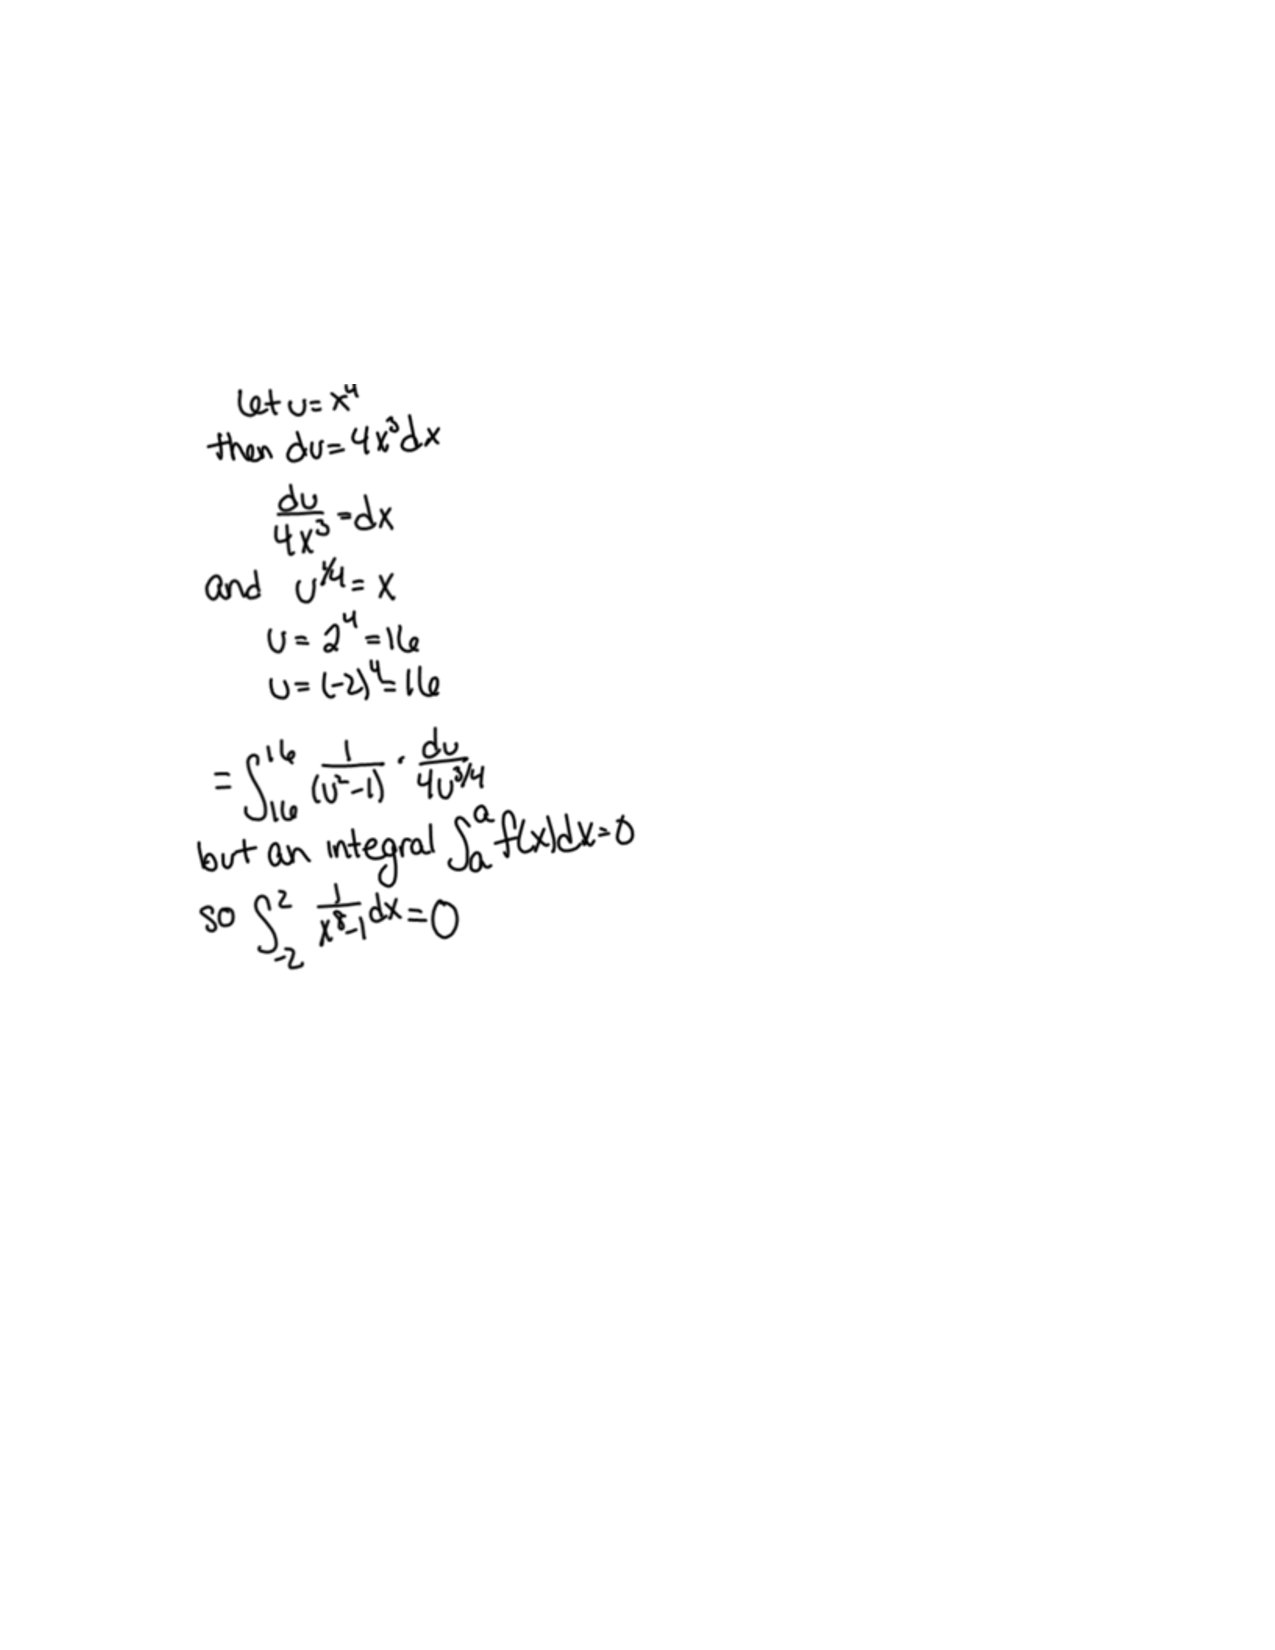
\includegraphics[trim= 170 420 250 180]{Figure1.pdf}
%\end{image}


\newcommand{\RR}{\mathbb R}
\renewcommand{\d}{\,d}
\newcommand{\dd}[2][]{\frac{d #1}{d #2}}
\renewcommand{\l}{\ell}
\newcommand{\ddx}{\frac{d}{dx}}
\newcommand{\dfn}{\textbf}
\newcommand{\eval}[1]{\bigg[ #1 \bigg]}

\usepackage{multicol}

\renewenvironment{freeResponse}{
\ifhandout\setbox0\vbox\bgroup\else
\begin{trivlist}\item[\hskip \labelsep\bfseries Solution:\hspace{2ex}]
\fi}
{\ifhandout\egroup\else
\end{trivlist}
\fi} %% we can turn off input when making a master document

\title{Recitation \#1 - Review of Substitution}  

\begin{document}
\begin{abstract}		\end{abstract}
\maketitle



\section{Warm up:}
Find the error in the following ``solution":

Find $\int_{-2}^2 \frac{1}{x^8 - 1} \d x$

	\begin{image}
	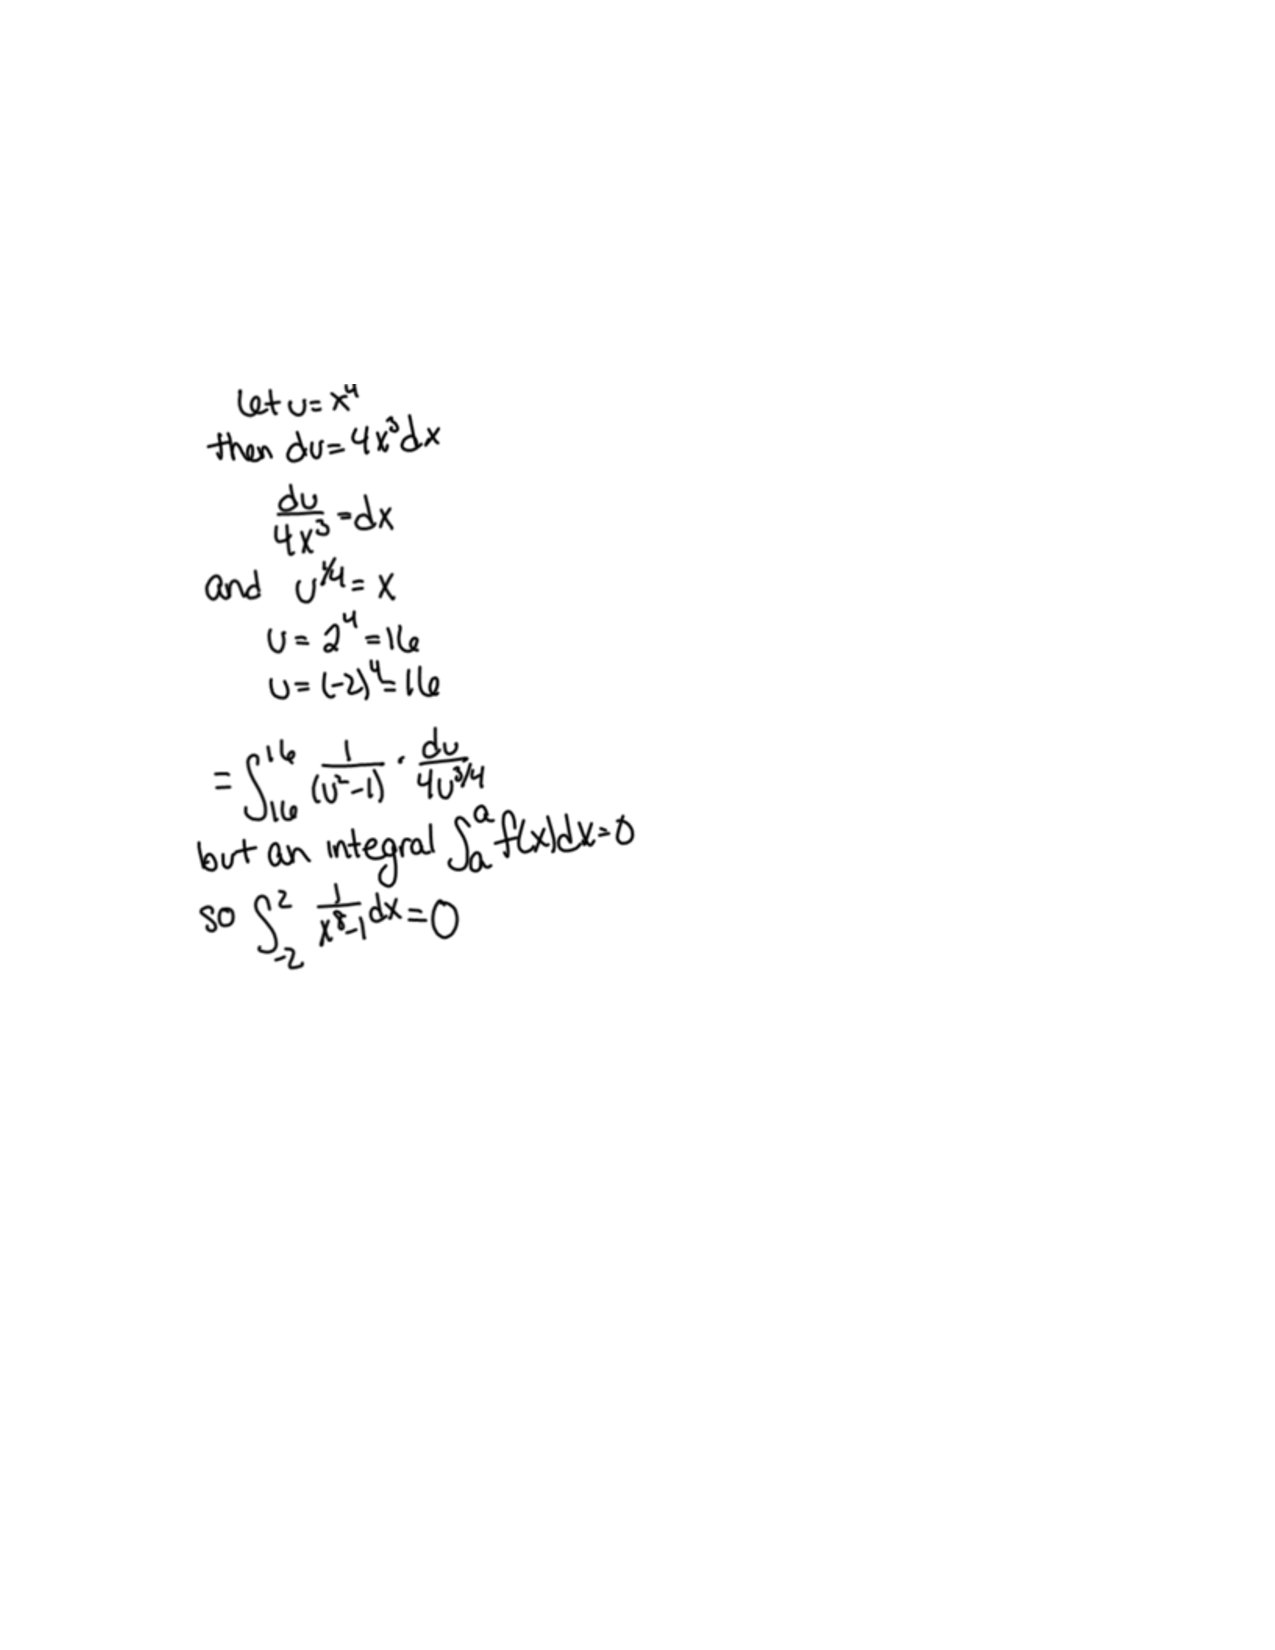
\includegraphics[trim= 120 320 350 180]{Figure1.pdf}
	\end{image}

	\begin{freeResponse}
	The error is that the function $\frac{1}{x^8-1}$ is not defined at $x=1$, and is therefore not continuous on the interval $[-2,2]$.
	\end{freeResponse}



\section{Group work:}



%problem 1
\begin{problem}
Compute the following integrals:

	\begin{enumerate}
	
	%part a
	\item  $\int 2t \sin \left( t^2 \right) \d t$
		\begin{freeResponse}
		Let $w=t^2$.  Then $\d w = 2t \d t$, and so
			\begin{align*}
			\int 2t \sin(t^2) \d t &= \int \sin(w) \d w  \\
			&= - \cos(w) + C  \\
			&= - \cos(t^2) + C.
			\end{align*}
		\end{freeResponse}
		
		
		
	%part b
	\item  $\int \sec^2(x) \tan(x) \d x$
		\begin{freeResponse}
		Let $u = \tan(x)$.  Then $\d u = \sec^2 (x) \d x$, and so
			\begin{align*}
			\int \sec^2(x) \tan(x) \d x &= \int u \d u  \\
			&= \frac{1}{2} u^2 + C  \\
			&= \frac{1}{2} \tan^2(x) + C.
			\end{align*}
		Note that the substitution $v=\sec(x)$ would also work to solve this problem.  
		It is a good exercise to work this out!
		\end{freeResponse}
		
		
		
	\end{enumerate}
		
		
\end{problem}







%problem 3
\begin{problem}
Compute the following integrals:

	\begin{enumerate}
	
	%part a
	\item  $\int \frac{x^2 }{1 + x^2} \d x$
		\begin{freeResponse}
		In general, when integrating a rational function where the degree of the numerator is greater than or equal to the degree
		of the denominator, you want to do long division to get the smallest possible degree in the numerator.  
		But watch this slick little trick:
			\begin{equation*}
			\frac{x^2}{1+x^2} = \frac{1 + x^2 - 1}{1+x^2} = \frac{1+x^2}{1+x^2} - \frac{1}{1+x^2} = 1 - \frac{1}{1+x^2}.
			\end{equation*}
		So
			\begin{align*}
			\int \frac{x^2 }{1 + x^2} \d x &= \int \left( 1 - \frac{1}{1+x^2} \right) \d x  \\
			&= x - \arctan(x) + C.
			\end{align*}
		I learned the trick above through tons and tons of practice solving integrals.  
		So guess what is a good idea for you to do before the final exam???
		\end{freeResponse}
		
		
		
	%part b
	\item  $ \int \frac{1+3x}{4+4x^2} \d x$
		\begin{freeResponse}
		First notice that
			\begin{equation*}
			\int \frac{1+3x}{4+4x^2} \d x = \frac{1}{4} \int \frac{1+3x}{1+x^2} \d x = \frac{1}{4} \int \left( \frac{1}{1+x^2} + \frac{3x}{1+x^2} \right) \d x.
			\end{equation*}
		The first integral is $\arctan(x)$, and so we have
			\begin{equation}\label{3b1}
			\int \frac{1+3x}{4+4x^2} \d x = \frac{1}{4} \arctan(x) + \frac{3}{4} \int \frac{x}{1+x^2} \d x.
			\end{equation}
		We can solve this second integral by substitution.  Let $u=1+x^2$.  Then $\d u = 2x \d x$ and $\frac{1}{2} \d u = x \d x$.  So
			\begin{equation}\label{3b2}
			\int \frac{x}{1+x^2} \d x = \frac{1}{2} \int \frac{1}{u} \d u = \frac{1}{2} \ln|u| +C = \frac{1}{2} \ln(1+x^2) + C.
			\end{equation}
		Plugging equation \eqref{3b2} into equation \eqref{3b1} yields
			\begin{equation*}
			\int \frac{1+3x}{4+4x^2} \d x = \frac{1}{4} \arctan(x) + \frac{3}{8} \ln(1+x^2) + C.
			\end{equation*}
		\end{freeResponse}
		
		
		
	\end{enumerate}
			
			
		
\end{problem}







%problem 6
\begin{problem}
Evaluate the following integrals:

	\begin{enumerate}
	
	%part a
	\item  $\int \frac{13x^7}{\sqrt{3x^4-5}} \d x$
		\begin{freeResponse}
		Let $v = 3x^4 - 5$.  Then
			\begin{align*}
			&\d v = 12 x^3 \d x  \\
			&x^4 = \frac{1}{3} (v + 5).
			\end{align*}
		So
			\begin{align*}
			\int \frac{13x^7}{\sqrt{3x^4-5}} \d x &= \frac{13}{12} \int \frac{(x^4)(12 x^3)}{\sqrt{3x^4-5}} \d x  \\
			&= \frac{13}{12} \int \frac{\frac{1}{3} (v+5)}{\sqrt{v}} \d v  \\
			&= \frac{13}{36} \int \left( v^{\frac{1}{2}} + 5v^{-\frac{1}{2}} \right) \d v  \\
			&= \frac{13}{36} \left( \frac{2}{3} v^{\frac{3}{2}} + 10 v^{\frac{1}{2}} \right) + C  \\
			&= \frac{13}{54} (3x^4-5)^{\frac{3}{2}} + \frac{65}{18} \sqrt{3x^4 - 5} + C.
			\end{align*}
		\end{freeResponse}
		
		
		
	%part b
	\item  $\int \frac{x^3}{x^2 - 3} \d x$
		\begin{freeResponse}
		Let $w = x^2 - 3$.  Then
			\begin{align*}
			&\d w = 2x \d x  \\
			&x^2 = w + 3.
			\end{align*}
		So
			\begin{align*}
			\int \frac{x^3}{x^2 - 3} \d x &= \frac{1}{2} \int \frac{(x^2)(2x)}{x^2 - 3} \d x  \\
			&= \frac{1}{2} \int \frac{w+3}{w} \d w  \\
			&= \frac{1}{2} \int \left(1 + \frac{3}{w} \right) \d w  \\
			&= \frac{1}{2} \left( w + 3 \ln|w| \right) + C  \\
			&= \frac{1}{2} \left( x^2 - 3 + 3\ln|x^2-3| \right) + C.
			\end{align*}
		\end{freeResponse}
		
		
		
	\end{enumerate}
			
			
	
\end{problem}
















	
	
	
	
	
	
	
	
	

	










								
				
				
	














\end{document} 


















